\section{Punto de Vista de Mapa de Capacidad}

El punto de vista del mapa de capacidades permite al arquitecto de la empresa crear una visión general estructurada de las capacidades de la empresa. Un mapa de capacidad típicamente muestra dos o tres niveles de capacidades en toda la empresa. Puede, por ejemplo, utilizarse como mapa de calor para identificar áreas de inversión. En algunos casos, un mapa de capacidades también puede mostrar los resultados específicos que ofrecen esas capacidades.

\subsection{Modelo de Mapa de Capacidad}
\begin{figure}[h!]
	\centering
	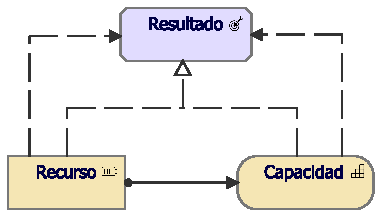
\includegraphics[width=.5\linewidth]{imgs/caso/MapaCapacidad}
	\caption{Modelo Mapa de Capacidad}
\end{figure}

En sínstesis, un recurso es un activo que es propiedad o está controlado por un individuo u organización. Por otra parte, una capacidad es una habilidad que posee un elemento de estructura activa, como una organización, una persona o un sistema. Y, finalmente, un curso de acción es un enfoque o plan para configurar algunas capacidades y recursos de la empresa, dispustos para la consecusión de un objetivo. \\

Aumentar el beneficio es un objetivo que puede descomponerse en varios otros objetivos: Disminuir los costos y aumentar los ingresos. El primero está relacionado con la estrategia de Operación Excelencia de la empresa, modelada como un curso de acción. Estos resultan en dos resultados: Disminución de los costos y pérdida de clientes, que influyen en los objetivos de manera positiva y negativa. Esto muestra una importante diferencia entre los objetivos y los resultados: no todos los resultados conducen a los resultados previstos.
Los cursos de acción se realizan por una serie de capacidades: Gestión y operaciones de TI y gestión de productos, y los recursos apropiados Recursos humanos y recursos de TI se asignan a las primeras.

\newpage

\subsection{Caso de Mapa de Capacidad}

\subsubsection{Resutlado 1: Mejores Investigadores e Investigaciones}

\begin{figure}[h!]
	\centering
	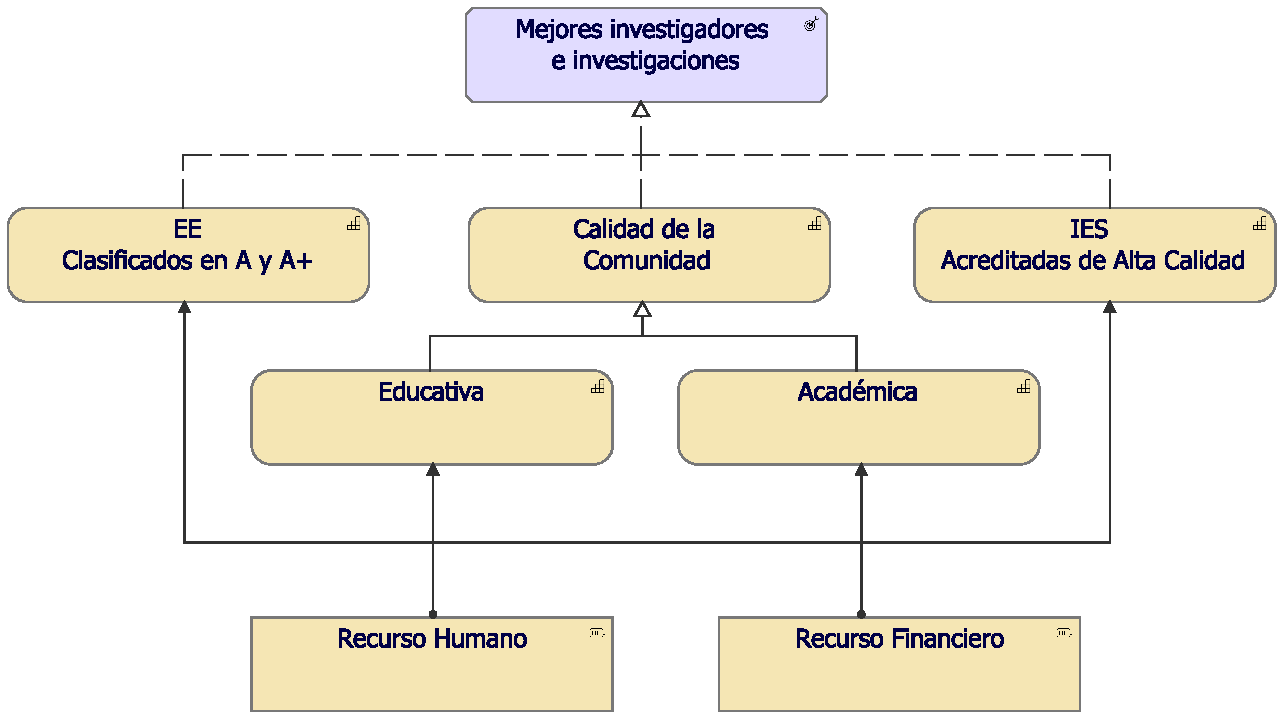
\includegraphics[width=1\linewidth]{imgs/modelo/estrategia/capacidad/1.pdf}
	\caption{Caso Mapa de Capacidad}
\end{figure}

Para dar alcance al resultado de obtener mejores investigadores y mejores investigaciones, el MEN como estructura activa se basa en las habilidades inmersas tanto en los Establecimientos Educativos de calificación A y A+ \footnote{\url{https://www.icfes.gov.co/documents/20143/193495/Clasificacion+de+establecimientos+y+sedes+Saber+11.pdf/2f177381-3c38-6b20-f5da-272dba42b412}}, los cuales representan la mayoría de los planteles registrados, así como las habilidades al interior de sus Instituciones de Educación Superior acreditadas de alta calidad. \\

No obstante, estas habilidades se encuentran arraigadas a la capacidad provista por la calidad de la comunidad, educativa y académica respectivamente. A saber, el activo más importante del MEN, el recurso humano; y que, junto al recurso financiero, conforman el punto de partida para el curso de acción de la organización.

\clearpage
\subsubsection{Resutlado 2: Generación de Estudiantes de Alta Calidad}

\begin{figure}[h!]
	\centering
	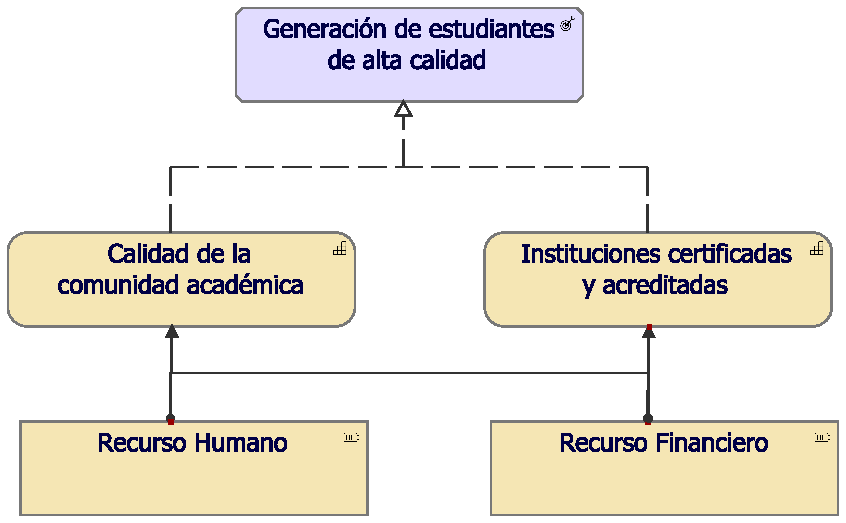
\includegraphics[width=.7\linewidth]{imgs/modelo/estrategia/capacidad/2.pdf}
	\caption{Caso Mapa de Capacidad}
\end{figure}

En en el marco de la \textbf{generación de estudiantes} de alta calidad, el MEN dispone de dos capacidades como lo son la calidad de la comunidad académica e instituciones certificadas y acreditadas que garantizan el desarrollo de procesos con altos estándares de calidad. Las cuales, junto con los recursos humano y financiero, se encuntran configurados dentro del curso de acción para la consecusión de dicho objetivo.